\chapter{MemoryStroop: Concept, Design and Implementation}
\label{ch:desenvolvimento}

In this chapter, we present the guidelines of our implementation with the requirements' analysis, the technical aspects of its development, and the general work  (the conduction of this research is only presented in the next chapter, `Experiment'). After presenting requirements' basis as we indicated in previous chapter, it is time to consolidate for validating it with its targeted final users, in this case, ADHD children. As we underlined before, a gamiefied application have to deal, to balance funny features with serious aims in order to turn practical but awful tasks more pleasant. This is the main principle of this thesis, that can be shown in every section of the present chapter, where we finally evaluate the core features.

\section{Requirements}

The requirements are based in the release of a previous gamified  application for ADHD children and in an idea collected from a scientific article of Psychology. First, it is necessary explain the contribution of the let worth foundations for the present work. As expressed other times before, our application, MemoryStroop is inspired by the research and the application made by S\'{e}rgio Villa \citep{Villa}. However, now we have a new and quite different application, although both share some similarities. To starts, the main contribution of Villa's work is its feedback of psychologists, computer science students and non-ADHD children the tested the game, name only ``Cores'' (Colors, in Portuguese). Villa submitted multiple-answer questionnaires of usability analysis in order to check quality mixed with some open questions in order to present the positive aspects and possible ameliorations to another features. 

\subsection{Requirement prospection}

In doing so, it were pointed, mainly in psychologists' opinions, some necessities to be achieved. On general, they approved and viewed with good eyes the use of the said software as mean of treatment, but some of them manifested the following points for improving in a near version of software: first, the gaming has too much conflicting stimuli in some of its levels, secondly a general performance report is needed and thirdly moving targets to player. To discuss and present these improvements, it is necessary before to present briefly the application itself. In summary, Villa's application implements a gaming centered in matching  (like the third test of John Ridley Stroop, but more influenced by Golden Stroop modality) of a color name to an ink, but, most of times in a situation of conflicting stimuli, mainly a conflict between the color name and its background ink. So, eight levels lets the player/patient from the simplest matching of a color name and its ink without any conflict in the first level, to a difficult scenario with a series of adverse stimuli in the last one.

\subsection{Defining requirements}

A general score with response time and hit rates is also implemented, satisfying the requirement expressed by the psychologists. Then, these requirements may be grouped and presented as a list of requirements, including the functional and non-functional ones, the latter are disposed according to the patterns of ISO9126's norms.


\begin{table}[h!] % The `h` means place the table here. The exclamation mark tells Latex to really try to place the table here. Use with caution! 
	
	\begin{center}
		\scalebox{0.85}{
			\begin{tabular}{ l  l  l  l }
				\hline
				\textbf{Number} & \textbf{As a <role>} & \textbf{As a <goal>} & \textbf{As a <result>} \\
				\hline \hline
				1.1 & Player & access menu & select new game\\
				1.2 & Player & give the name & write his/her name \\
				1.3 & System & generate board 
				& dispose `stroop' memory cards \\
				2.1 & Player & seek color name combination  & pass levels\\
				2.2 & System &  manage hits and mistakes & improve difficulty slightly \\
				2.3  & Player & advance levels until the end & conclude gaming \\
				3.1 & Psychologist & see statistics &  must see player's name and numbers
				 \\
				\hline \hline
			\end{tabular}}
		\end{center}
		\label{tab:highuserstories}
		\caption{Table for the all Functional Requirements}
	\end{table}

\begin{table}[h!]
Table \ref{tab:NonFuncReq} lists the non-functional requirements to develop the application. 

\begin{center}
	\scalebox{0.6}{%
		\begin{tabular}{ l  l  l }
			\hline
			\textbf{Number} & \textbf{Requirements} & \textbf{Quality in use} \\
			\hline \hline	
			\textbf{Functionality} & & \\
			F1 & The player should have only option to follow the game levels & Consistency\\
			F2 & The system should each level's statistics & Consistency\\
			\hline
			\textbf{Usability} & & \\
			U1 & A new player should be able to use the system after less than 5 minutes training & Learnability\\
			U2 & The system should be perceived as easy to use by at least 85\% of its users & Understandability \\
			\hline
			\textbf{Maintainability} & & \\
			M1 & The system should be easy to extend and modify & Changeability\\ % Make measurable
			\hline
			\textbf{Portability} & & \\
			P1 & The system should run on the majority of used android devices without additional resources & Installability\\
			\hline \hline
		\end{tabular} }
	\end{center}
	\label{tab:NonFuncReq}
	\caption{Table for all Non-functional Requirements}
	\end{table}

\subsection{Technologies for software Development}

The employed technologies are only the basic infrastructure for software development. The codification of the mobile software was made in Java programming language driven for Android mobile operating system. It was used the Android Studio framework in version 1.5.1 for the development, implementing gradle, the package manager for android projects and some other frameworks too, the lint prototypes validator and OpenJDK 7 (Java Developer Kit) for Java programming language infrastructure on a Debian 8 (Jessie) operating system desktop for development. \footnote{Although Google warns that using Open JDK instead the Oracle proprietary JDK may let problems to application, but no problemas are related to this in our application.} 

As differences of traditional Java for desktops or other mobile platform, Android has some specific functions, as directed to call device resources or sensors, and runs in another virtual machine than common Java, the Dalvik Virtual Machine. Android has a stack of operating system levels, beginning from a linux kernel, passing to a device-components layer and other levels until arriving to a, as we can see in figure exposed below.

\begin{figure}[htp]
	\begin{center}
		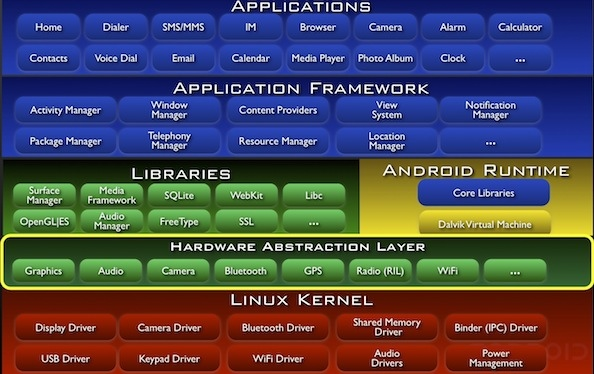
\includegraphics[scale=1.5]{chapters/desenvolvimento/img/android.png}
		\caption{Android operating system layers.}
		\label{Android-Schema}
	\end{center}
\end{figure}

The Android environment was chosen, especially, because it is the platform currently most used around the World, particularly in Brazil, where our study was designed and most of 80\% of mobile devices are Android-based, as we have been said in our Introduction. The native application approach, against other types of hybrid approaches like cross-compile one, is adopted here as way for exploring all potentialities of the native devices standard computational resources. In this way, it will so difficult to develop many native applications driven for each mean mobile device's operating system, like IOs or Windows Phone, because it will demand more time and resources that a single coursework subject could afford.

So, our application is designed for Android environments to achieve a grater number of potential users. Besides, the experiment designed for this research comprises only a controlled and reduced group of people, since the software is an experimental application, although an older version is offered, for free, on Google Play App store or others, which contains dozens of millions of mobile applications of the most different finalities. Android platform are also more accessible to develop than other platform like IOs or Blackberry, for whom it is necessary a considerable number of environment requirements, like the exigence of a computer Mac for programming in Objective-C or Swift (languages that implements applications to IOs), that difficult the programming process. So that, there is a couple of reasons to adopt the Android environment to develop the application of this research, mainly, its popularity in Brazil and its relative practicality for development. 

The application is compatible from Android ``Kitkat'' (version 4.4) to the most recent versions (the most stable recent version in moment which is version 6 called ``Marshmallow''), that yields a compatibility ration in order of about 74\% of Android devices on a word-wide perspective, according to recent data \citep{android-official}. Our implementation also is driven to treat different resolutions of devices, using scalable images and other strategies, as we will discuss soon. In this case, tablets and smart-phones with different dimensions like Galaxy Nexus or Moto G and son could run as well the application presented here. To develop the game core features it is used the Libgdx Java library and engine. It is as free software engine that allows anyone program simple 2D or 3D games for various platforms, including Android. So, the proposed application, Mememory Stroop, combine libgdx to some native android native code and directives that are proper of this system. Libdgx offers a large set of facilities to better develop games for Android. One of the, maybe the most important, is its simplicity of operations and basic project's architecture and high integration by Java programming language syntax shared by both. Additionally, Android Studio IDE could easily manage Libgdx projects with gradle and implement extra native code as well. Furthermore, this Java game engine has powerful resources to implement game textures, sprites, events, loops, input-getting, abstract and non-abstract screens, and other features that let game development and gamification more accessible to non-specialists of that area.

\section{General features and application architecture}
As mentioned before, Villa's ADHD gamification comprise multiple conflict situation in game that appeared undesirable to some of the psychologists. So these extent set of conflict mechanisms that is replaced by only two conflicting stimuli of classical stroop test a fixed memory game board, in order to promote a more focused set of stimuli. It was implemented in the present application. So, that's why our application is called MemoryStroop. The number of levels were reduced to four, beginning to the 2x2 board with card without conflicting stimuli in the first level to a Stroop conflict in the next level, that increases board to 4x4, 8x8 and 16x16 boards in each level. All negative stimuti that remained on old version, like ``game over'' event, were removed too: only positive stimuli such as commemorative music effects are implemented. 

Below it is possible see the game implementation's architecture of Libgdx Java classes and extra native android class, that implements PDF exportation of game statistical data.

\section{Summary}

At this moment of the coursework, the point was to present to reader how it were set the computational and technical aspects of MemoryStroop. Thus the first necessity referred to the definition of requirements, which came from a previous application and research \citep{Villa}, improving some of main features presented by the psychologists about that application and research. The main requirement of those psychologists is the necessity to offer a limited set of conflicting stimuli during the Stroop Effect during the game. So far so good the functional and non-functional  requirements that